% 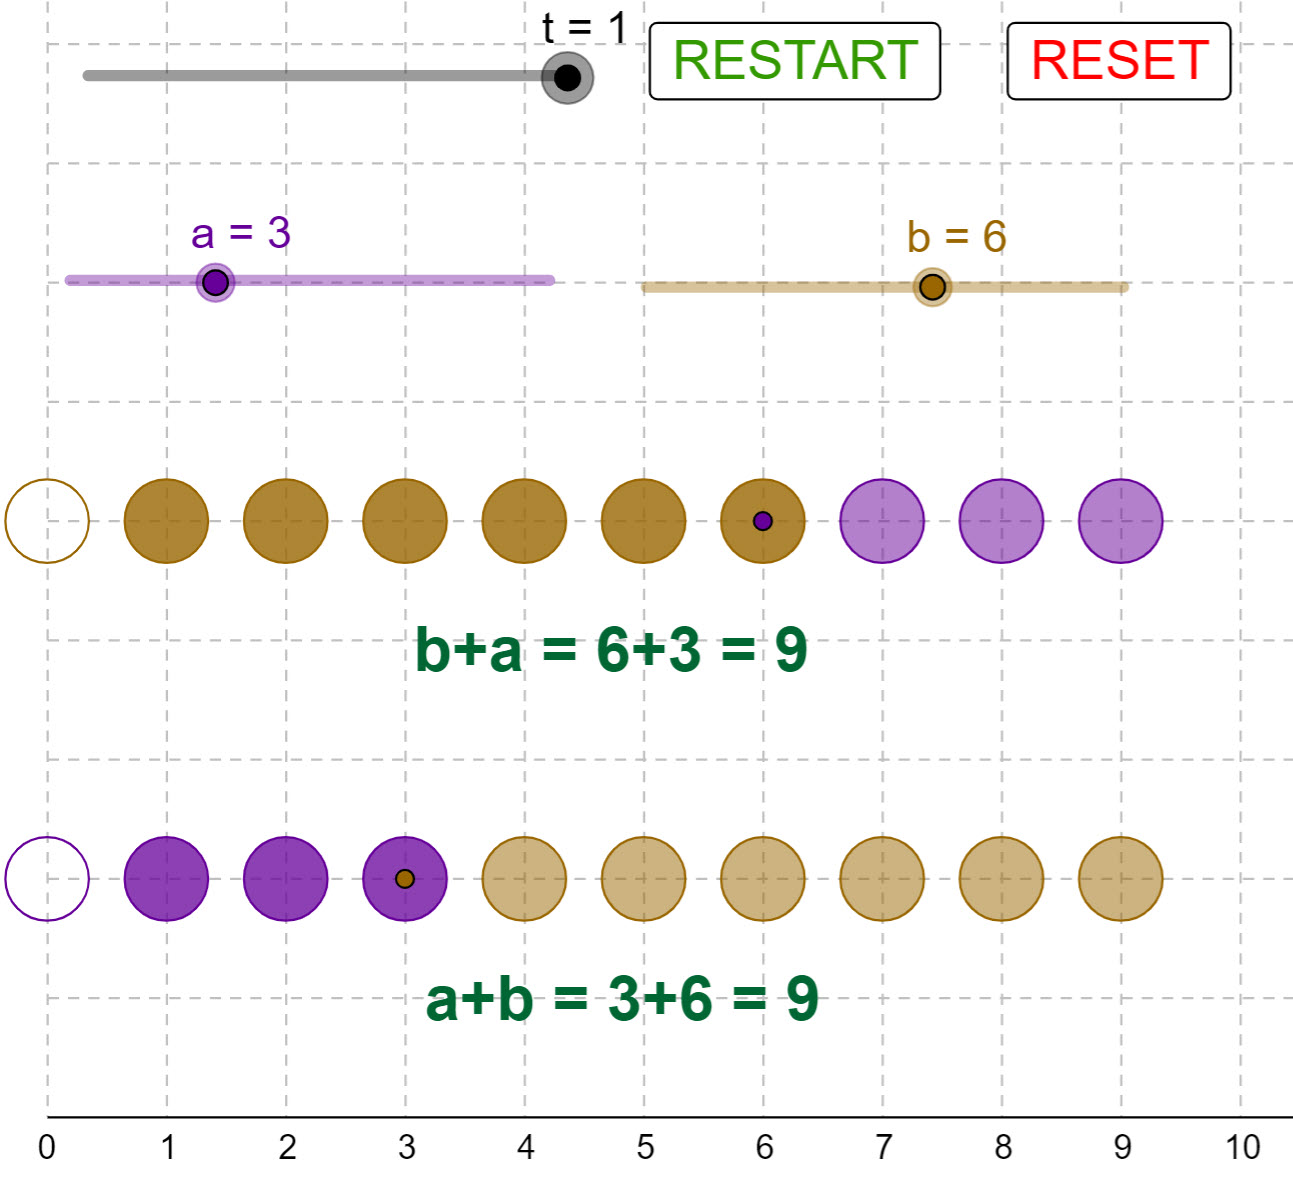
\includegraphics[width=20mm]{Images/sm-001.jpg}

\chapter{\protect\hyperlink{chap:\thechapter}{Properties of Arithmetic}}
\addtocontents{toc}{\protect\hypertarget{chap:\thechapter}{}}



\section{Why Start with Arithmetic?}
Arithmetic refers to the basics of adding, subtracting, multiplying, dividing, and (maybe) more exotic things like squares and square roots.
But you already know how to add, subtract, multiply, and divide  so why do we have an entire chapter on the properties arithmetic?  You probably learned most of these basics already. The hardest thing that you usually do in arithmetic is “word problems” like “If Jenny has 5 apples and Timmy has 7 apples, then how many apples do they have together?” As you get older, the numbers get bigger, but the problems don’t really get much harder. Arithmetic is great when trying to solve simple problems like counting apples. But when the problems get more complicated we will need Algebra.


\begin{problem}
This is a problem
\end{problem}


\begin{connection}
The properties and vocabulary you focus on here will be used in Algebra and Sets and so are not confined to use with arithmetic. The Number Strand prepares us for and leads on to the Algebra Strand and so in post-primary school we study Number with concepts and language that will form a bridge between Number and Algebra. Some books name this bridge \textbf{prealgebra} . What is prealgebra?  Prealgebra is the bridge between arithmetic and algebra.
\end{connection}






 



To take a simple example, you can use arithmetic to show that\[ 2 \times (3 + 5) = (2 \times 3) + (2 \times 5), \]because the left side equals $2 \times 8$, which is 16, and the right side equals $6 + 10$, which is also 16. But algebra gives us the much more general tool that\[ a \times (b + c) = (a \times b) + (a \times c), \]no matter what numbers $a$, $b$, and $c$ are. While this implies that the letters are \textbf{variables} $a$, $b$, and $c$ might even become \textbf{expressions} and    \textbf{sets} and an exotic number called a \textbf{complex numbers} \footnote{These are numbers that you don't have to worry about or recognise until you are in TY and Leaving Certificate maths!} Even more generally, “$+$” and “$\times$” might not mean addition and multiplication as you think of them now, but instead might represent more complicated mathematical operations when we study \textbf{sets}  so rest assured careful thinking and mastering of the vocabulary we use here is very important.

Our initial goal,lay down the rules of arithmetic, and to give you some ideas as to why these rules are true. Once you know the rules, you’ll be ready to start thinking algebraically.

Also, by the time you start reading this book, you are mathematically mature enough to start thinking about not just how to perform various calculations, but why the techniques used in those calculations work. Understanding why mathematics works is the key to solving harder problems. If you only understand how techniques work but not why they work, you’ll have a lot more difficulty modifying those techniques to solve more complicated problems. So, throughout this book, we will rarely just tell you how something works–we’ll usually show you why it works.

By the end of this chapter, you should be able to explain why the following computations are true:

\section{Basic computation}




\section{Commutative Law of Addition}


\begin{figure*}[h!]
   \centering
    \href{https://www.geogebra.org/m/CsDdkudm}{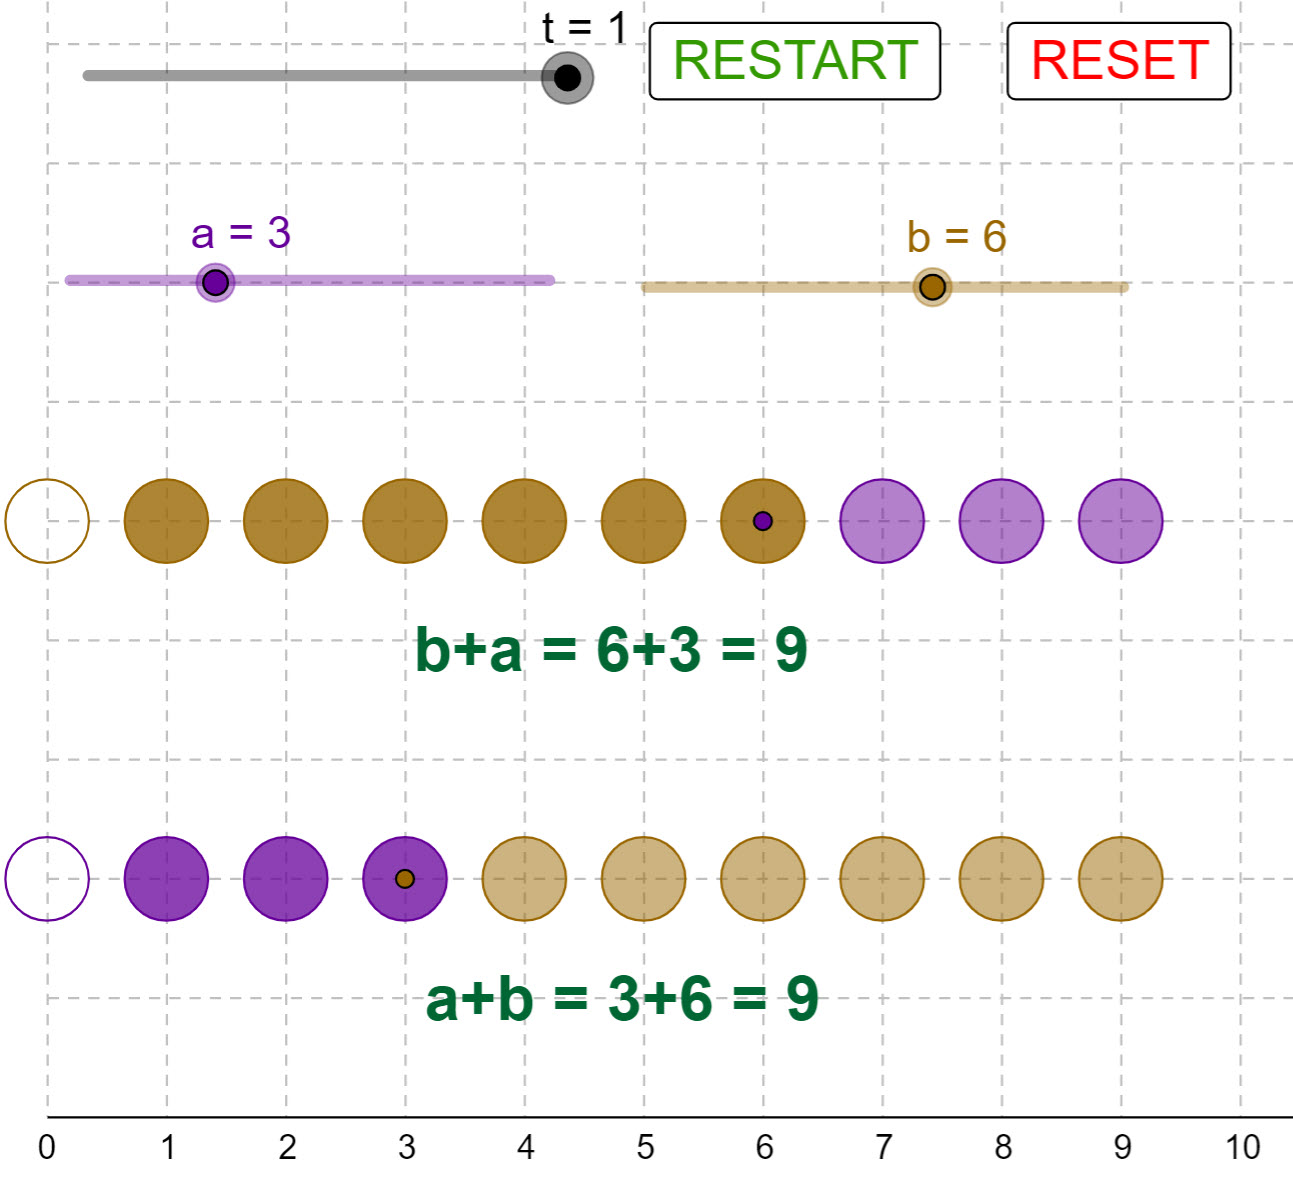
\includegraphics[width=.6\textwidth]{Images/sm-001.jpg}}
    \caption{\href{https://www.geogebra.org/m/CsDdkudm}{Click anywhere to explore the Commutative Law of Addition.}}
\end{figure*}














\section{Commutative Law of Addition}
\begin{figure}%[4]
    \centering
    \href{https://www.geogebra.org/m/CsDdkudm}{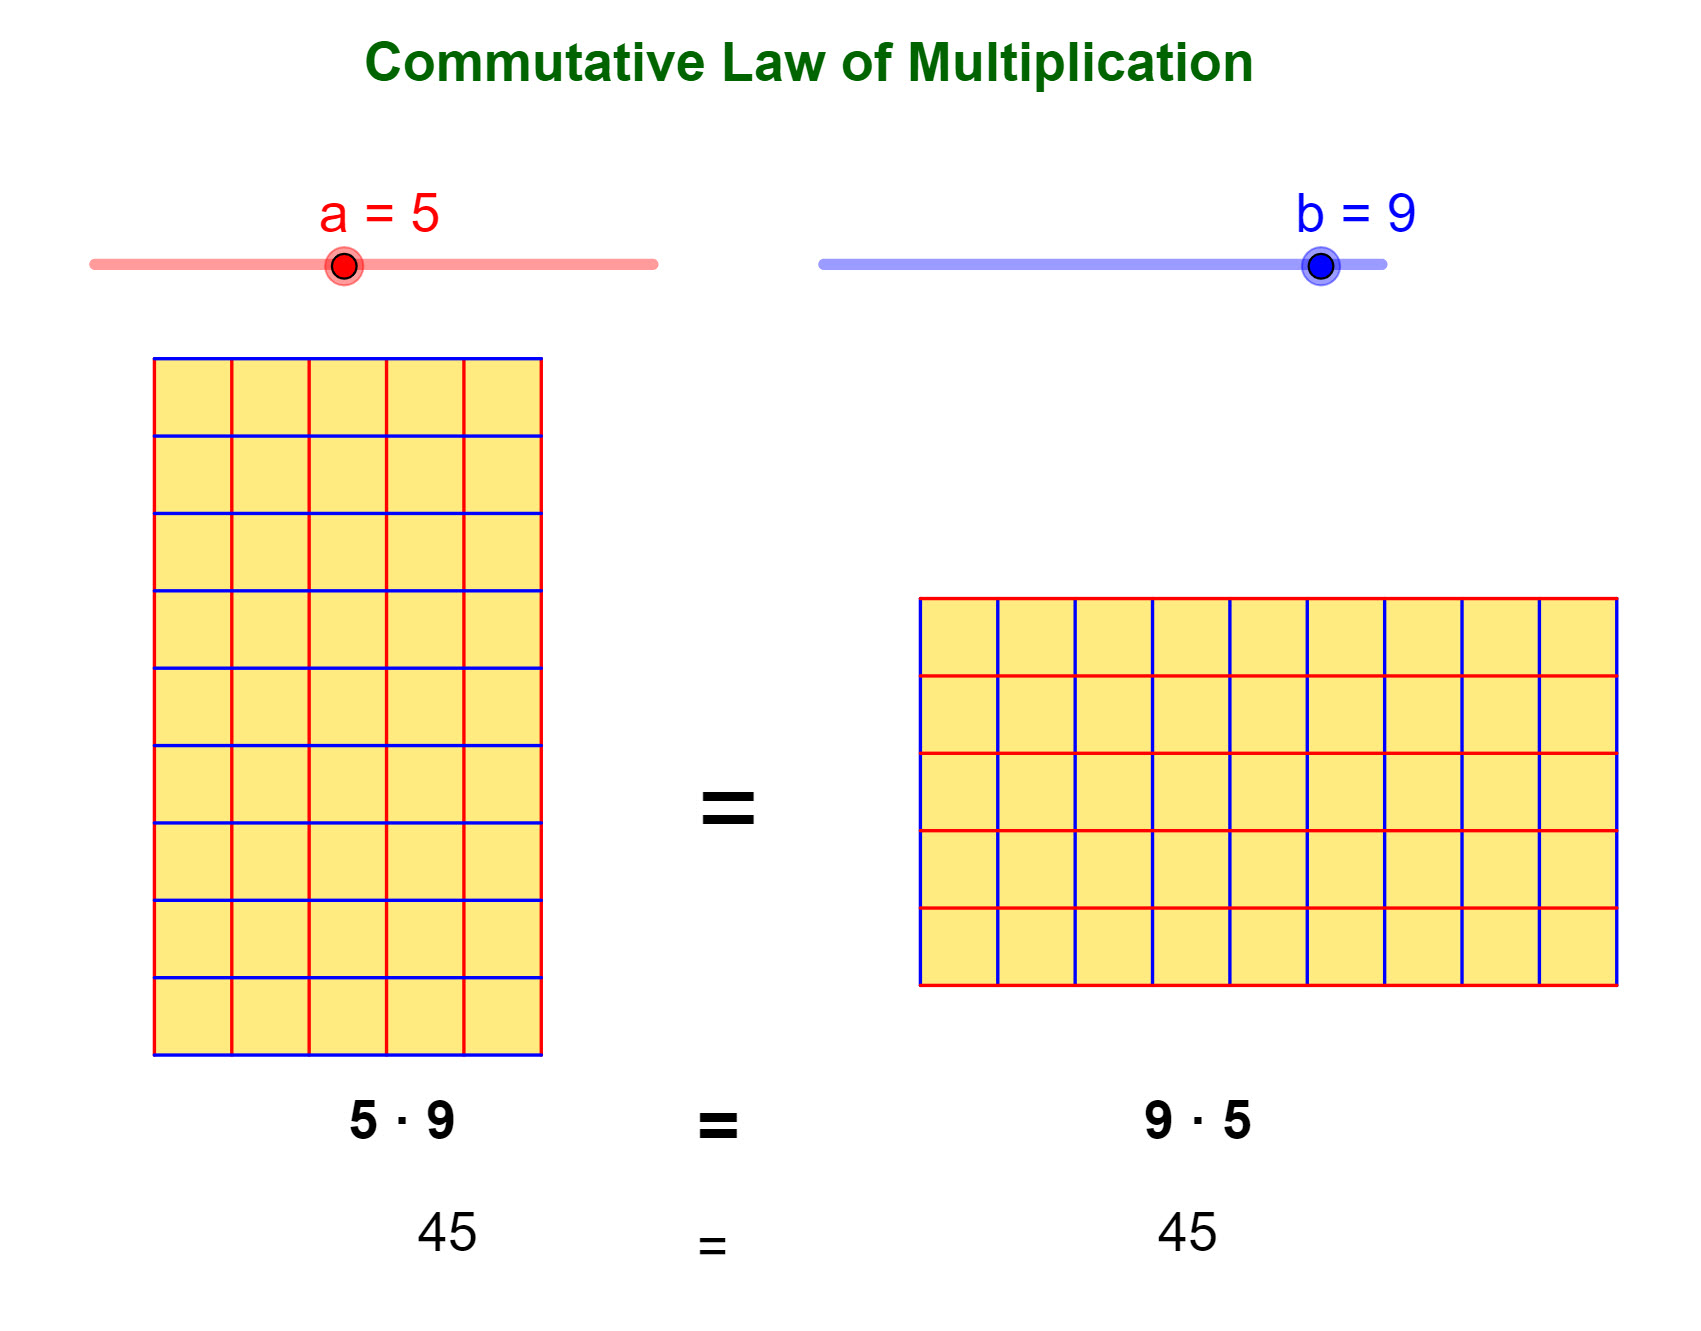
\includegraphics[width=.6\textwidth]{Images/sm-000.jpg}}
    \caption{\href{https://www.mathopenref.com/trianglecircumcircle.html}{Click anywhere to explore the circumcentre and circumcircle of a triangle.}}
\end{figure}



\section{perform mixed arithmetic operations of positive
integers involving multiple levels of brackets}












\section{understand the concept of power}




\section{Enrichment Material marked with asterisks$^*$}

\section{HL only material is underlined}



\section{Expanded Media}


\section{Comparing Completion and Reduction}
N.3 investigate situations involving proportionality so that they can:
a. use absolute and relative comparison where appropriate
b. solve problems involving proportionality including those involving currency conversion
and those involving average speed, distance, and time